\chapter{Introduction to Project}\hrule
\label{Chapter:1}
% =====================================================================================================
\section{Overview}

This project sequentially applies a set of Mysql techniques to gain insights from the Instagram Database.Mysql Environoment analysis of this data will benefit the business processes of the Instagram.
 \\
\\
This project deals with designing and implementing a system for handling the information of behavioral
evaluations. An Analyst schedules subject evaluations and then analyses the recorded behaviors that
occur during specified collection periods. The evaluations provide data that can be analyzed in order to
develop plans that will help treat the subject as needed.
The collection periods or appointments as they have been called in our project are scheduled by the
analyst, conducted by the therapist and data during these appointments is collected by a collector
present. Our system also implements an admin user who is required for user management and behavior
data management. 
 \section {Exitsing System}
 
 As day by day, the data used increases and therefore a better way of handling such a huge amount of data is becoming a hectic task. The traditional approach of data storage File System Storage.FFS is for unstructured data  as well as structured data.It stores the average size of data.
 \\
 \\
  When a size of data is too big for complex processing and storing or not easy to define the relationships between the data, then it becomes difficult to save the extracted information in an FSS with a coherent relationship.
  \\
  \\
  By the above comparison, we have come to know that MYSQL is the best technique for handling Big Data compared to that of FSS.
\section{Functional Requirements}
\begin{itemize}
	\item Setup of MYSQL Environment.
	\item PC needs to have atleast 4 GB Ram and atleast 100GB  of external usable memory.
	\item PC should have Ubuntu 16.4v or Windows 7 or above.
\end{itemize}
\section{Feasibility Study}
A feasibility study is used to determine the viability of an idea, such as ensuring a project is legally and technically feasible as well as economically justifiable. It tells us whether a project is worth the investment—in some cases, a project may not be doable. There can be many reasons for this, including requiring too many resources, which not only prevents those resources from performing other tasks but also may cost more than an organization would earn back by taking on a project that isn’t profitable.\\
\\
The application is fully feasible. It just needs a working internet connection,PC have atleast 4 GB RAM. It is fully feasible if it is also deployed on a large scale.\\
The Project can also be upgraded further and can be deployed on large scale depending upon the need of business plan.\\
\begin{enumerate}
	\item \textbf{Technical Feasibility :} The Project is fully feasible on technical terms. I have PC and required 4 GB Ram for development purpose.\\
	I will use MYSQL Environment to deploy backend as it is frees.\\
	The version control system is completely free and the website Github.com is also free for Open Source Projects.
   \item \textbf{Economic Feasibility :} The Project is fully economically feasible as it has free and open source tools being used while developing the system.\\
   \item \textbf{Legal Feasibility :} The Project doesn't violates any legal rights and will credit the author of open Source Library used while developing the project.\\
   The project will be available in open source under \textbf{GPLv3} license.\\
   \\
   \textbf{What is GPLv3 License?}
   \begin{itemize}
   	\item The source code must be made public whenever a distribution of the software is made.
   	\item Modifications of the software must be released under the same license.
   	\item Changes made to the source code must be documented.
   	\item If patented material was used in the creation of the Project, it grants the right for users to use it. If the user sues anyone over the use of the patented material, they lose the right to use the Project.\\
   \end{itemize}
 
   \item \textbf{Operational Feasibility : } As the Project satisfies the functional and non functional requirements, the Project will be fully operational once it releases.
   
   \item \textbf{Scheduling Feasibility : } The project release targets for different versions are practical and have plenty of time develop and debug the Project before release.
\end{enumerate}

\section{Objectives of the Project }
The main objective of this project is given below-
\begin{itemize}
	\item finding 5 oldest users.
	\item what day of the weeks do most users register on?
    \item find the users who have never posted any photos.
    \item find most likes on single photo.
	\item HOW many times does the average user post ?
	\item What are the top 5 most commanly used hashtags ?

	
\end{itemize}




\chapter{Product Design}\hrule
\label{Chapter:3}
% =====================================================================================================

\section{Product Perspective}
This Project utilizes Data Classification to examine a dataset related with Instagram Database.“Data Classification” is the use of MYSQL techniques to organize datasets into related sub-populations, not previous specified in the dataset. This can uncover hidden characteristics within data, and identify hidden categories that new data belongs within.
\section{Table Structure}
The dataset examined by this Project was collected from a Instagram Databases.I use MYSQL Database for this project. Here we describe the all table-
\\
\textbf{users}
	 \begin{figure}[h!]
	 	\centering
	 	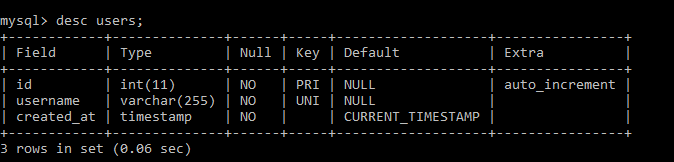
\includegraphics[width=0.75\linewidth]{user.png}
	 	\caption{users table}
	 \end{figure}
 \\
 \textbf{follows}
 \begin{figure}[h!]
 	\centering
 	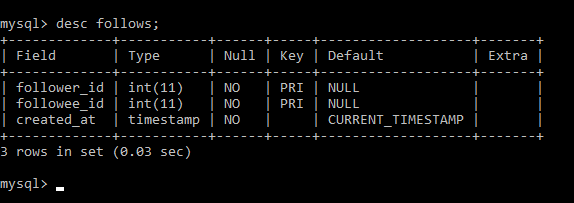
\includegraphics[width=0.75\linewidth]{follows.png}
 	\caption{follows table}
 \end{figure}
\\
\textbf{likes}
\begin{figure}[h!]
	\centering
	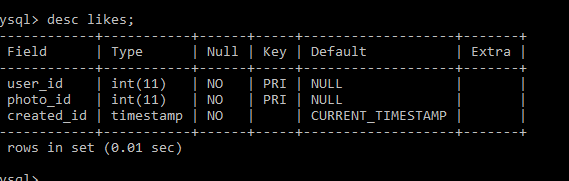
\includegraphics[width=0.75\linewidth]{likes.png}
	\caption{likes table}
\end{figure}
\\
\textbf{comments}
\begin{figure}[h!]
	\centering
	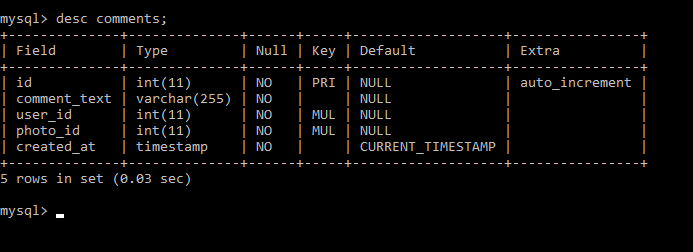
\includegraphics[width=0.75\linewidth]{comments.png}
	\caption{comments table}
\end{figure}\\
\textbf{photos}
\begin{figure}[h!]
	\centering
	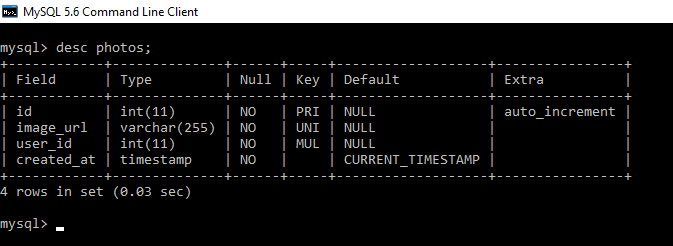
\includegraphics[width=0.75\linewidth]{photos.png}
	\caption{photos table}
\end{figure}\\
\textbf{photos-tags}
\begin{figure}[h!]
	\centering
	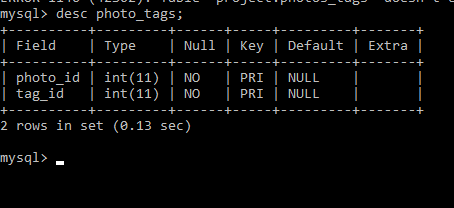
\includegraphics[width=0.75\linewidth]{photo_tag.png}
	\caption{photo tags table}
\end{figure}
\\
\textbf{tags}
\begin{figure}[h!]
	\centering
	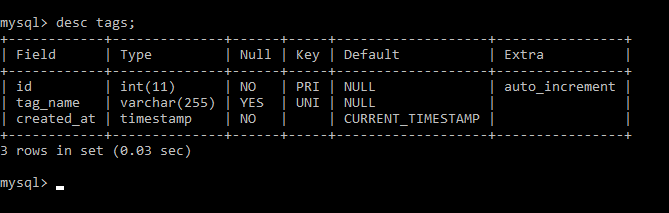
\includegraphics[width=0.75\linewidth]{tags.png}
	\caption{tags table}
\end{figure}
\\

\section{E-R MOdel}
Entity Realationship model of table is given below-
\begin{figure}[h!]
	\centering
	\includegraphics[width=0.75\linewidth]{er.png}
	\caption{E-R Model}
	\label{fig:E-R Model}
\end{figure}
\section{Specific Requirements}
\begin{itemize}
	\item PC have ubuntu 16.4,windows 7.0 or above os.
	\item Working internet connection.
	\item Minimum 4 GB Ram and 100 GB external memory.
\end{itemize}
\chapter{Development and Implementation}\hrule
\label{Chapter:4}
% =====================================================================================================
\section{Data Importing}

In order to begin processing the Instagram Datasets are imported into the MySql environment and stored in MySql. After import of the data, we find the datasets contains lots of records. 

\section{Introduction to Language}
\textbf{SQL}
\\
SQL is a standard language for storing, manipulating and retrieving data in databases.SQL can execute queries against a database.It can retrieve data from a database.It can insert records in a database.It can update records in a database.It can delete records from a database.It can create new databases.SQL can create new tables in a database.It can create stored procedures in a database.SQL can create views in a database.SQL can set permissions on tables, procedures, and views.

\section{Implementation with ScreenShots}
\\
\begin{figure}[h!]
	\centering
	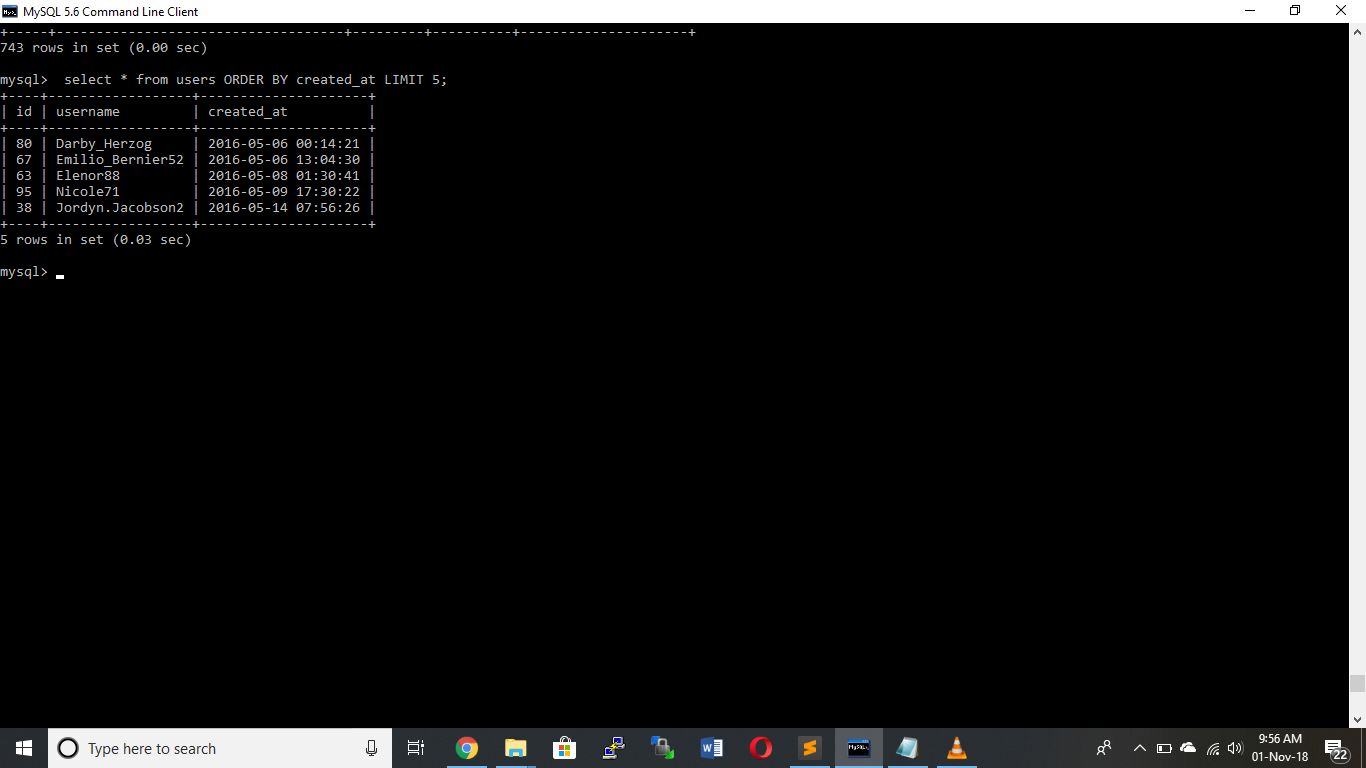
\includegraphics[width=0.75\linewidth]{sc1.png}
	\caption{5 oldest users}
\end{figure}
\begin{figure}[h!]
	\centering
	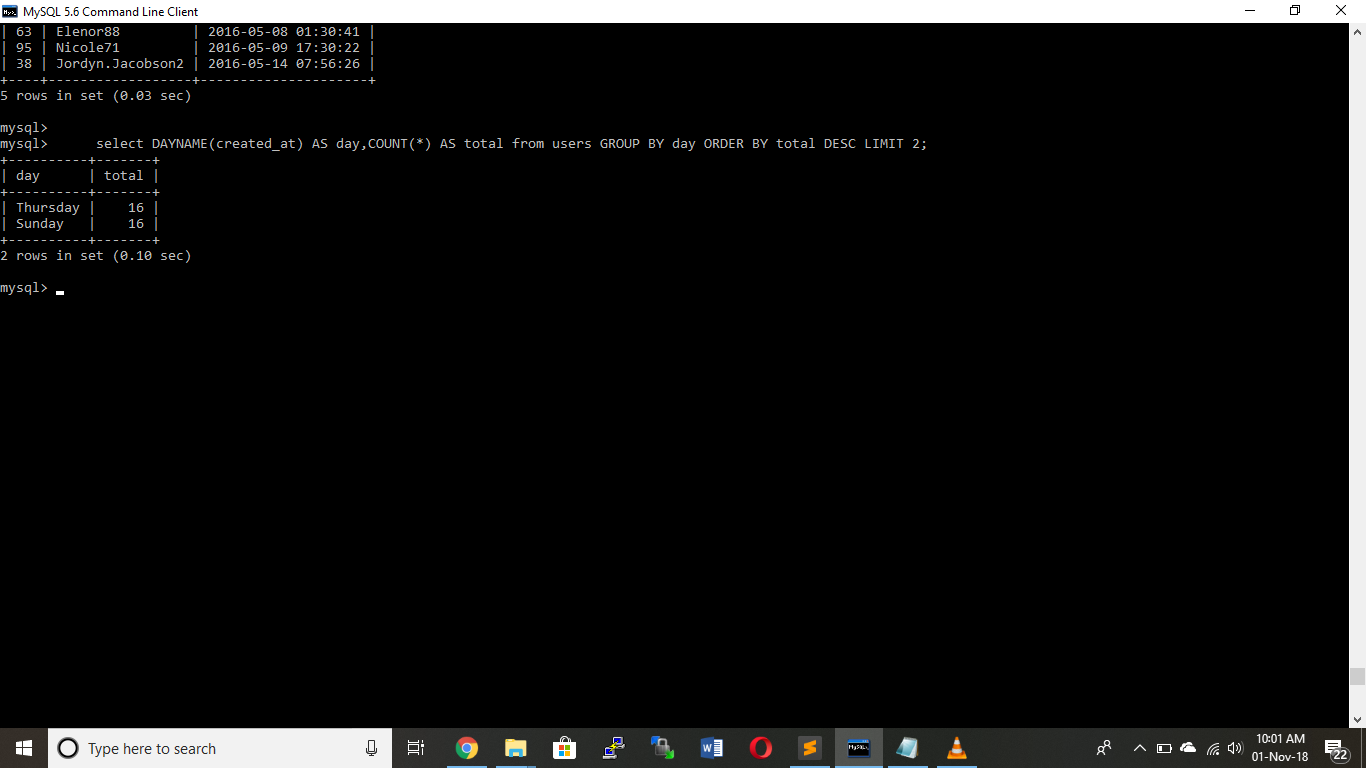
\includegraphics[width=0.75\linewidth]{sc2.png}
	\caption{day of weeks do most users register}
\end{figure}
\begin{figure}[h!]
	\centering
	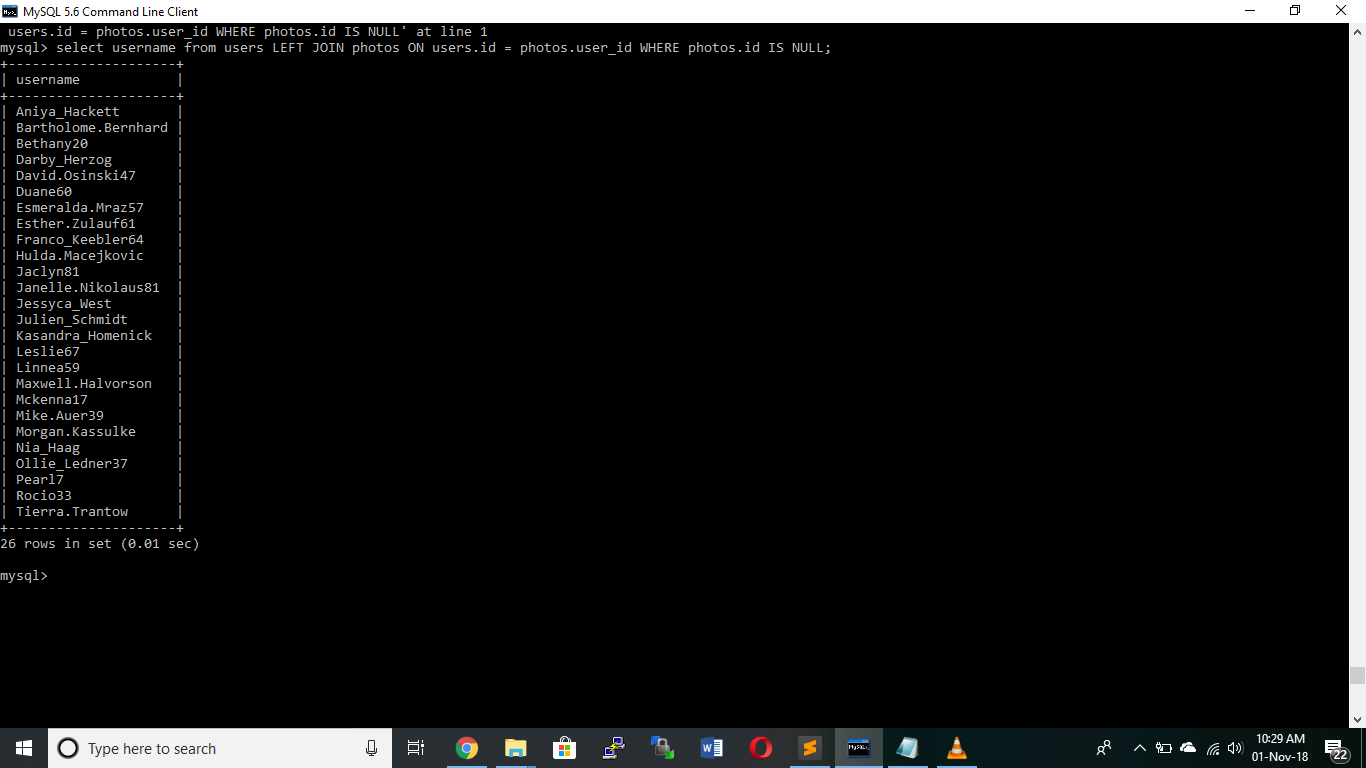
\includegraphics[width=0.75\linewidth]{sc3.png}
	\caption{user who have never posted any photos}
\end{figure}
\begin{figure}[h!]
	\centering
	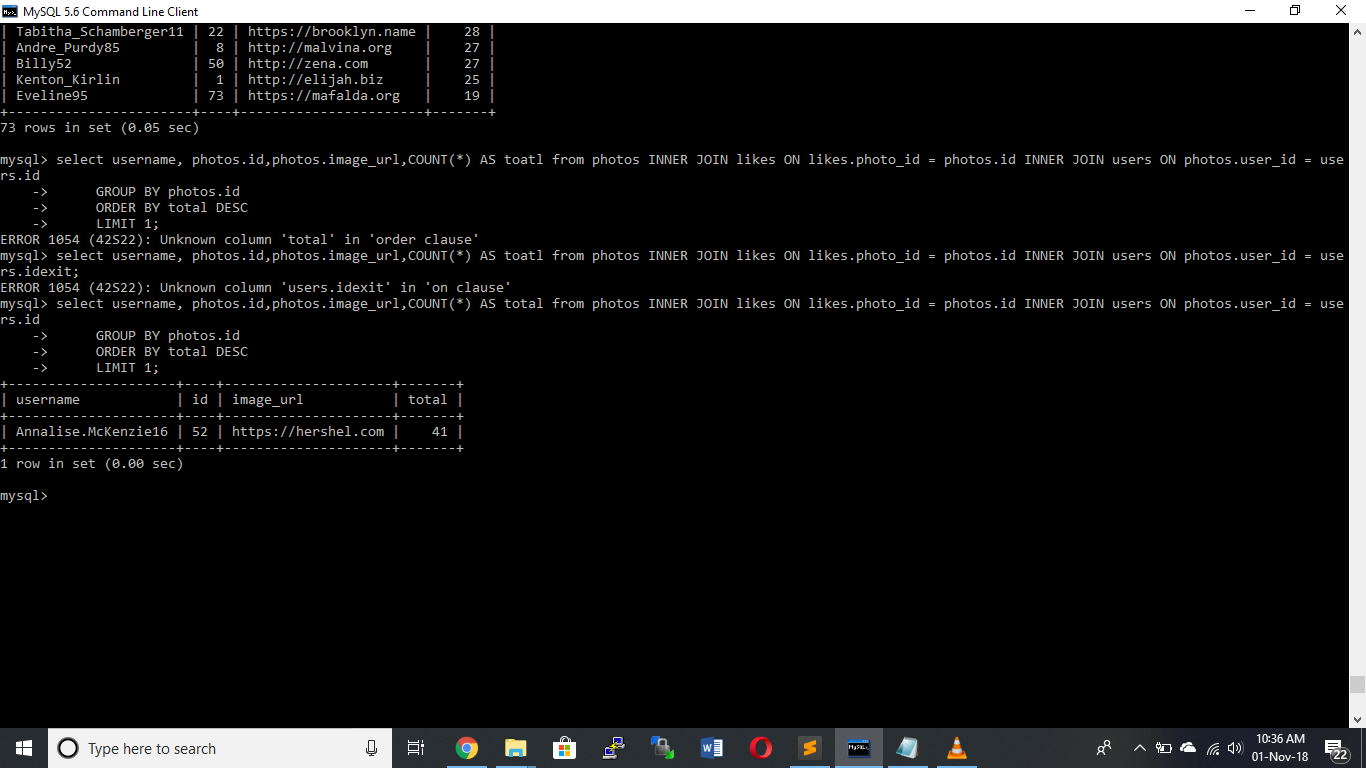
\includegraphics[width=0.75\linewidth]{sc4.png}
	\caption{most likes on single photo}
	
\end{figure}
\begin{figure}[h!]
	\centering
	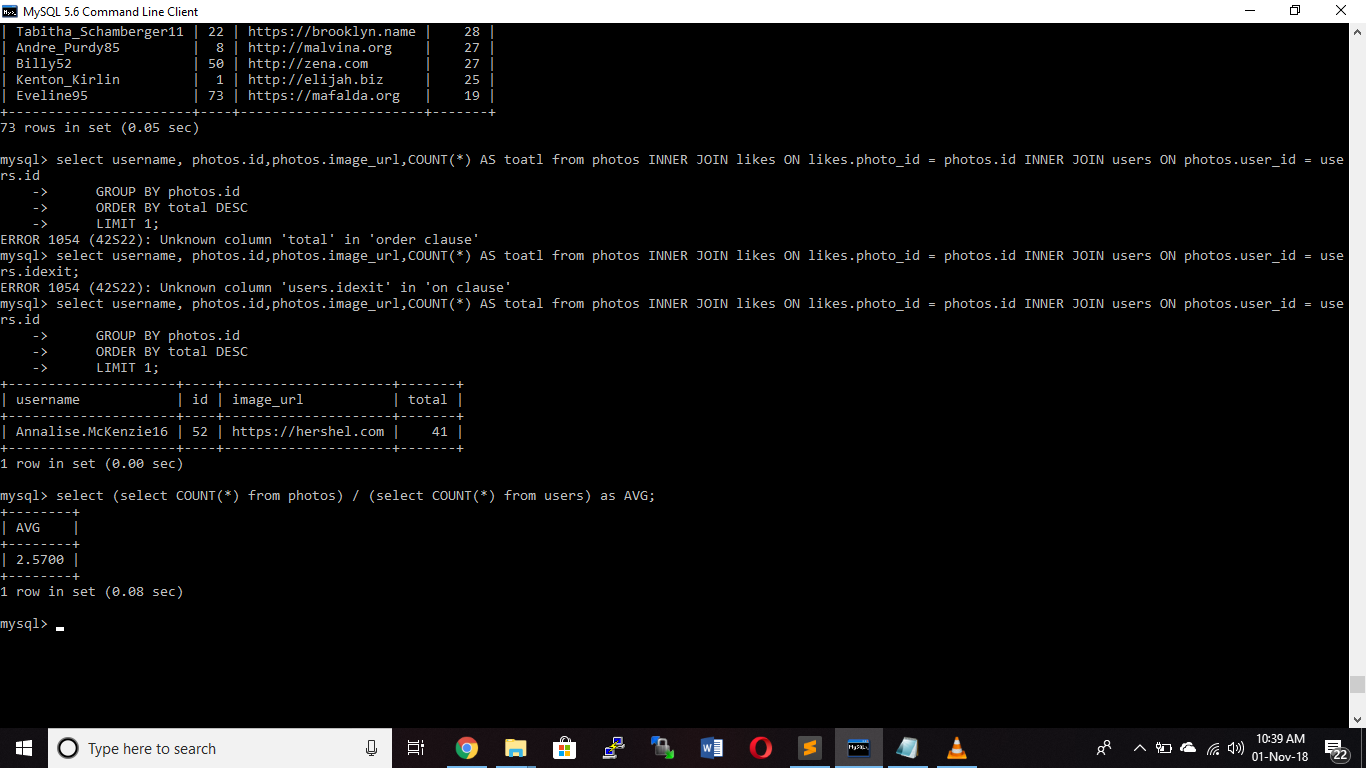
\includegraphics[width=0.75\linewidth]{sc5.png}
	\caption{average user post}
	
\end{figure}\\
\begin{figure}[h!]
	\centering
	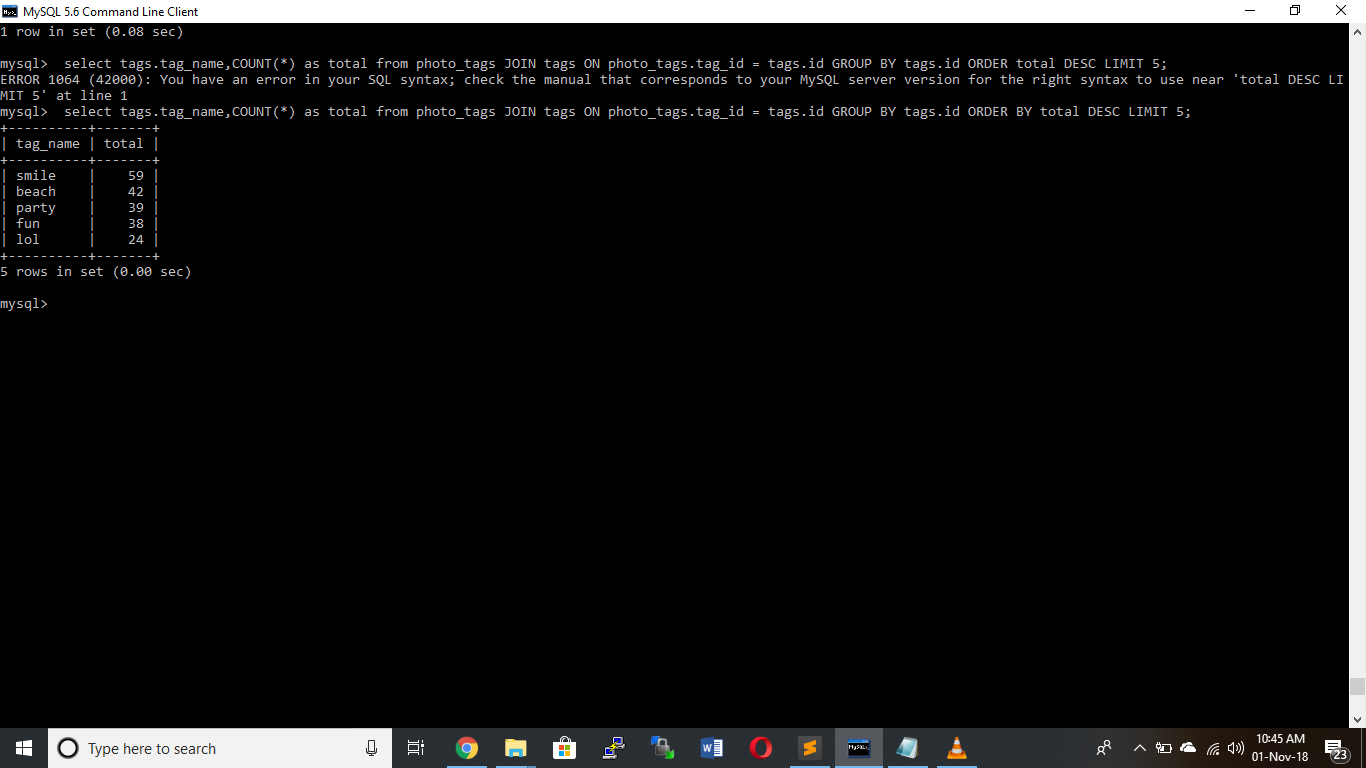
\includegraphics[width=0.75\linewidth]{sc6.png}
	\caption{5 commanly used hashtags}
\end{figure}\\	
\chapter{Conclusion and Future Scope}\hrule
\label{Chapter:5}
% =====================================================================================================
\section{Conclusion}
This project has implemented all the features of Rdbms to handle Instagram Database and analyze to increases Instagram business.
\section{Future Scope}
The Project has been keeping in mind of future feature additions.\\
Due to Digitalization and other factors have made things accessible while simultaneously making it difficult to keep data structured and well-managed.\\
The Project has main moto to increase revenue of Instagram and make them increases marketing. I hope,this Project will achieve its aim of development and will generate a great revenue for Instagram.
\chapter{Refrences}\hrule
\label{Chapter:6}
% =====================================================================================================
\begin{enumerate}
	\item https://www.mysql.com/ [accesed on 02/10//018]
	\item https://www.w3schools.com/sql/default.asp [accesed on 08/10//018]
	\item https://www.tutorialspoint.com/sql/ [accesed on 20/10//018]
	\item https://stackoverflow.com/questions/tagged/sql-server [accesed on 25/10//018]
	\item https://repository.genmymodel.com/JamesonReden/InstagramSchema [accesed on 30/10//018]
	\item https://www.draw.io/ [accesed on 03/11//018]
\end{enumerate}